% RDM truncation, after ITransverse.jl Fig. 6(a) and Fig. 7.
% (a) fixes the notation: a canonical tensor contracted with its conjugate is the identity.
% (b) is the statement that makes the truncation local: the eigenvalues of the reduced density
%     matrix at a cut are the squared singular values of the orthogonality centre alone.
% A tensor and its conjugate are the same shape in a lighter and a darker shade.
%
% Standalone: compiles to imgs/truncation.pdf.
% Inline:     with \usepackage{standalone}, % RDM truncation, after ITransverse.jl Fig. 6(a) and Fig. 7.
% (a) fixes the notation: a canonical tensor contracted with its conjugate is the identity.
% (b) is the statement that makes the truncation local: the eigenvalues of the reduced density
%     matrix at a cut are the squared singular values of the orthogonality centre alone.
% A tensor and its conjugate are the same shape in a lighter and a darker shade.
%
% Standalone: compiles to imgs/truncation.pdf.
% Inline:     with \usepackage{standalone}, % RDM truncation, after ITransverse.jl Fig. 6(a) and Fig. 7.
% (a) fixes the notation: a canonical tensor contracted with its conjugate is the identity.
% (b) is the statement that makes the truncation local: the eigenvalues of the reduced density
%     matrix at a cut are the squared singular values of the orthogonality centre alone.
% A tensor and its conjugate are the same shape in a lighter and a darker shade.
%
% Standalone: compiles to imgs/truncation.pdf.
% Inline:     with \usepackage{standalone}, % RDM truncation, after ITransverse.jl Fig. 6(a) and Fig. 7.
% (a) fixes the notation: a canonical tensor contracted with its conjugate is the identity.
% (b) is the statement that makes the truncation local: the eigenvalues of the reduced density
%     matrix at a cut are the squared singular values of the orthogonality centre alone.
% A tensor and its conjugate are the same shape in a lighter and a darker shade.
%
% Standalone: compiles to imgs/truncation.pdf.
% Inline:     with \usepackage{standalone}, \input{imgs/truncation}.
\documentclass[tikz,border=3pt]{standalone}
\usepackage{amsmath,amssymb,braket,graphicx}
\usetikzlibrary{arrows.meta,shapes.geometric}

\definecolor{ketc}{RGB}{150,215,240}
\definecolor{brac}{RGB}{60,130,175}
\definecolor{ctrk}{RGB}{250,200,150}
\definecolor{ctrb}{RGB}{225,140,60}

\newcommand{\DX}{0.64}
\newcommand{\DY}{0.27}
\newcommand{\ST}{0.44}

\newcommand{\Dhh}{0.21}   % half-height of a tensor
\newcommand{\Dbb}{0.21}   % straight body, so the D is as wide as it is tall

% D-shaped tensors centred at (#1,#2), filled #3; \dR has its flat edge left, \dL right
\newcommand{\dR}[3]{%
  \filldraw[fill=#3, draw=black, line width=1.1pt]
    ({#1-(\Dbb+\Dhh)/2},{#2-\Dhh}) -- ({#1+(\Dbb-\Dhh)/2},{#2-\Dhh})
    arc[start angle=-90, end angle=90, radius=\Dhh]
    -- ({#1-(\Dbb+\Dhh)/2},{#2+\Dhh}) -- cycle;}
\newcommand{\dL}[3]{%
  \filldraw[fill=#3, draw=black, line width=1.1pt]
    ({#1+(\Dbb+\Dhh)/2},{#2-\Dhh}) -- ({#1-(\Dbb-\Dhh)/2},{#2-\Dhh})
    arc[start angle=-90, end angle=-270, radius=\Dhh]
    -- ({#1+(\Dbb+\Dhh)/2},{#2+\Dhh}) -- cycle;}

\newcommand{\bigpar}[1]{\scalebox{1.1}[4.6]{$#1$}}

\begin{document}
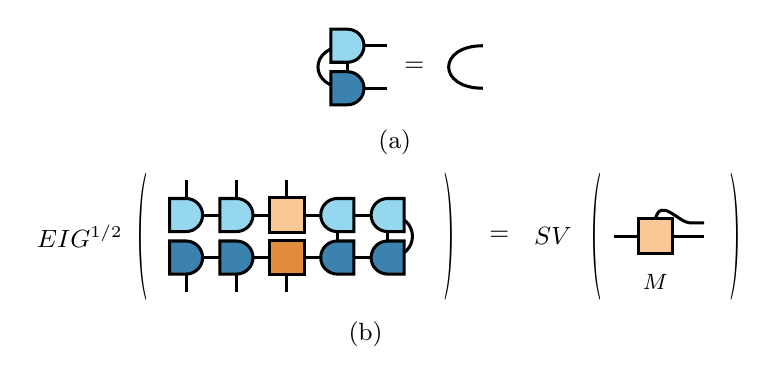
\begin{tikzpicture}[
    bond/.style={draw=black, line width=1.1pt},
    Sq/.style={rectangle, draw=black, line width=1.1pt, minimum size=4.4mm, inner sep=0pt},
    tag/.style={font=\small},
    idx/.style={font=\footnotesize},
  ]

  %% ================= (a) the canonical condition, centred =================
  \begin{scope}[xshift=2.05cm, yshift=2.15cm]
    \draw[bond] (0,\DY) .. controls (-0.50,\DY) and (-0.50,-\DY) .. (0,-\DY);
    \draw[bond] (0,\DY) -- (0,-\DY);
    \draw[bond] (0,\DY) -- (0.50,\DY);
    \draw[bond] (0,-\DY) -- (0.50,-\DY);
    \dR{0}{\DY}{ketc}
    \dR{0}{-\DY}{brac}
    \node[tag] at (0.85,0) {$=$};
    \draw[bond] (1.72,\DY) .. controls (1.14,\DY) and (1.14,-\DY) .. (1.72,-\DY);
    \node[tag] at (0.6,-0.95) {(a)};
  \end{scope}

  %% ================= (b) the RDM spectrum is local =================
  \node[tag] at (-1.35,0) {$EIG^{1/2}$};
  \node at (-0.55,0) {\bigpar{(}};

  % the reduced density matrix at a cut: left block open, right block traced
  \foreach \r/\s/\f/\g in {1/\DY/ketc/ctrk, -1/-\DY/brac/ctrb} {
    \draw[bond] (0,\s) -- ({4*\DX},\s);
  }
  \foreach \i in {0,1,2} {
    \draw[bond] (\i*\DX,\DY)  -- (\i*\DX,{\DY+\ST});
    \draw[bond] (\i*\DX,-\DY) -- (\i*\DX,{-\DY-\ST});
  }
  \foreach \i in {3,4} { \draw[bond] (\i*\DX,\DY) -- (\i*\DX,-\DY); }
  \draw[bond] ({4*\DX},\DY) .. controls ({4*\DX+0.42},\DY) and ({4*\DX+0.42},-\DY)
              .. ({4*\DX},-\DY);

  \foreach \i in {0,1} {
    \dR{\i*\DX}{\DY}{ketc}
    \dR{\i*\DX}{-\DY}{brac}
  }
  \node[Sq, fill=ctrk] at ({2*\DX},\DY)  {};
  \node[Sq, fill=ctrb] at ({2*\DX},-\DY) {};
  \foreach \i in {3,4} {
    \dL{\i*\DX}{\DY}{ketc}
    \dL{\i*\DX}{-\DY}{brac}
  }

  \node at ({4*\DX+0.78},0) {\bigpar{)}};
  \node[tag] at ({4*\DX+1.42},0) {$=$};
  \node[tag] at ({4*\DX+2.10},0) {$SV$};
  \node at ({4*\DX+2.65},0) {\bigpar{(}};

  % the orthogonality centre alone. The physical leg bends round to run parallel to the right bond:
  % the two indices are grouped, which is what turns M into a matrix for the SVD.
  \begin{scope}[xshift={(4*\DX+3.40)*1cm}]
    \draw[bond] (-0.52,0) -- (0.62,0);
    \draw[bond] (0,0.22) .. controls (0.07,0.50) and (0.30,0.17) .. (0.44,0.17) -- (0.62,0.17);
    \node[Sq, fill=ctrk] at (0,0) {};
    \node[idx, anchor=north] at (0,-0.36) {$M$};
  \end{scope}
  \node at ({4*\DX+4.42},0) {\bigpar{)}};

  \node[tag] at ({2*\DX+1.0},-1.25) {(b)};

\end{tikzpicture}
\end{document}
.
\documentclass[tikz,border=3pt]{standalone}
\usepackage{amsmath,amssymb,braket,graphicx}
\usetikzlibrary{arrows.meta,shapes.geometric}

\definecolor{ketc}{RGB}{150,215,240}
\definecolor{brac}{RGB}{60,130,175}
\definecolor{ctrk}{RGB}{250,200,150}
\definecolor{ctrb}{RGB}{225,140,60}

\newcommand{\DX}{0.64}
\newcommand{\DY}{0.27}
\newcommand{\ST}{0.44}

\newcommand{\Dhh}{0.21}   % half-height of a tensor
\newcommand{\Dbb}{0.21}   % straight body, so the D is as wide as it is tall

% D-shaped tensors centred at (#1,#2), filled #3; \dR has its flat edge left, \dL right
\newcommand{\dR}[3]{%
  \filldraw[fill=#3, draw=black, line width=1.1pt]
    ({#1-(\Dbb+\Dhh)/2},{#2-\Dhh}) -- ({#1+(\Dbb-\Dhh)/2},{#2-\Dhh})
    arc[start angle=-90, end angle=90, radius=\Dhh]
    -- ({#1-(\Dbb+\Dhh)/2},{#2+\Dhh}) -- cycle;}
\newcommand{\dL}[3]{%
  \filldraw[fill=#3, draw=black, line width=1.1pt]
    ({#1+(\Dbb+\Dhh)/2},{#2-\Dhh}) -- ({#1-(\Dbb-\Dhh)/2},{#2-\Dhh})
    arc[start angle=-90, end angle=-270, radius=\Dhh]
    -- ({#1+(\Dbb+\Dhh)/2},{#2+\Dhh}) -- cycle;}

\newcommand{\bigpar}[1]{\scalebox{1.1}[4.6]{$#1$}}

\begin{document}
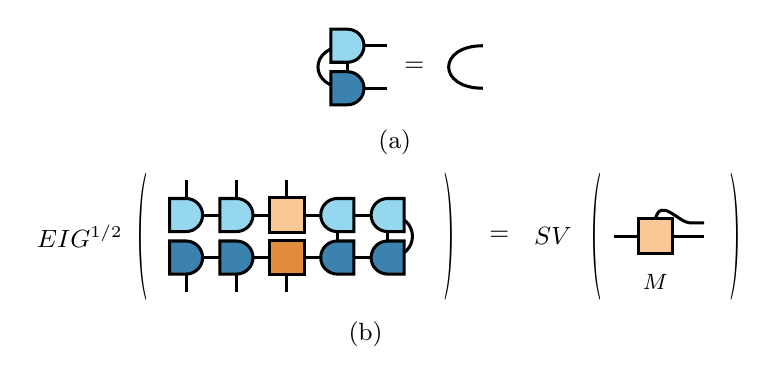
\begin{tikzpicture}[
    bond/.style={draw=black, line width=1.1pt},
    Sq/.style={rectangle, draw=black, line width=1.1pt, minimum size=4.4mm, inner sep=0pt},
    tag/.style={font=\small},
    idx/.style={font=\footnotesize},
  ]

  %% ================= (a) the canonical condition, centred =================
  \begin{scope}[xshift=2.05cm, yshift=2.15cm]
    \draw[bond] (0,\DY) .. controls (-0.50,\DY) and (-0.50,-\DY) .. (0,-\DY);
    \draw[bond] (0,\DY) -- (0,-\DY);
    \draw[bond] (0,\DY) -- (0.50,\DY);
    \draw[bond] (0,-\DY) -- (0.50,-\DY);
    \dR{0}{\DY}{ketc}
    \dR{0}{-\DY}{brac}
    \node[tag] at (0.85,0) {$=$};
    \draw[bond] (1.72,\DY) .. controls (1.14,\DY) and (1.14,-\DY) .. (1.72,-\DY);
    \node[tag] at (0.6,-0.95) {(a)};
  \end{scope}

  %% ================= (b) the RDM spectrum is local =================
  \node[tag] at (-1.35,0) {$EIG^{1/2}$};
  \node at (-0.55,0) {\bigpar{(}};

  % the reduced density matrix at a cut: left block open, right block traced
  \foreach \r/\s/\f/\g in {1/\DY/ketc/ctrk, -1/-\DY/brac/ctrb} {
    \draw[bond] (0,\s) -- ({4*\DX},\s);
  }
  \foreach \i in {0,1,2} {
    \draw[bond] (\i*\DX,\DY)  -- (\i*\DX,{\DY+\ST});
    \draw[bond] (\i*\DX,-\DY) -- (\i*\DX,{-\DY-\ST});
  }
  \foreach \i in {3,4} { \draw[bond] (\i*\DX,\DY) -- (\i*\DX,-\DY); }
  \draw[bond] ({4*\DX},\DY) .. controls ({4*\DX+0.42},\DY) and ({4*\DX+0.42},-\DY)
              .. ({4*\DX},-\DY);

  \foreach \i in {0,1} {
    \dR{\i*\DX}{\DY}{ketc}
    \dR{\i*\DX}{-\DY}{brac}
  }
  \node[Sq, fill=ctrk] at ({2*\DX},\DY)  {};
  \node[Sq, fill=ctrb] at ({2*\DX},-\DY) {};
  \foreach \i in {3,4} {
    \dL{\i*\DX}{\DY}{ketc}
    \dL{\i*\DX}{-\DY}{brac}
  }

  \node at ({4*\DX+0.78},0) {\bigpar{)}};
  \node[tag] at ({4*\DX+1.42},0) {$=$};
  \node[tag] at ({4*\DX+2.10},0) {$SV$};
  \node at ({4*\DX+2.65},0) {\bigpar{(}};

  % the orthogonality centre alone. The physical leg bends round to run parallel to the right bond:
  % the two indices are grouped, which is what turns M into a matrix for the SVD.
  \begin{scope}[xshift={(4*\DX+3.40)*1cm}]
    \draw[bond] (-0.52,0) -- (0.62,0);
    \draw[bond] (0,0.22) .. controls (0.07,0.50) and (0.30,0.17) .. (0.44,0.17) -- (0.62,0.17);
    \node[Sq, fill=ctrk] at (0,0) {};
    \node[idx, anchor=north] at (0,-0.36) {$M$};
  \end{scope}
  \node at ({4*\DX+4.42},0) {\bigpar{)}};

  \node[tag] at ({2*\DX+1.0},-1.25) {(b)};

\end{tikzpicture}
\end{document}
.
\documentclass[tikz,border=3pt]{standalone}
\usepackage{amsmath,amssymb,braket,graphicx}
\usetikzlibrary{arrows.meta,shapes.geometric}

\definecolor{ketc}{RGB}{150,215,240}
\definecolor{brac}{RGB}{60,130,175}
\definecolor{ctrk}{RGB}{250,200,150}
\definecolor{ctrb}{RGB}{225,140,60}

\newcommand{\DX}{0.64}
\newcommand{\DY}{0.27}
\newcommand{\ST}{0.44}

\newcommand{\Dhh}{0.21}   % half-height of a tensor
\newcommand{\Dbb}{0.21}   % straight body, so the D is as wide as it is tall

% D-shaped tensors centred at (#1,#2), filled #3; \dR has its flat edge left, \dL right
\newcommand{\dR}[3]{%
  \filldraw[fill=#3, draw=black, line width=1.1pt]
    ({#1-(\Dbb+\Dhh)/2},{#2-\Dhh}) -- ({#1+(\Dbb-\Dhh)/2},{#2-\Dhh})
    arc[start angle=-90, end angle=90, radius=\Dhh]
    -- ({#1-(\Dbb+\Dhh)/2},{#2+\Dhh}) -- cycle;}
\newcommand{\dL}[3]{%
  \filldraw[fill=#3, draw=black, line width=1.1pt]
    ({#1+(\Dbb+\Dhh)/2},{#2-\Dhh}) -- ({#1-(\Dbb-\Dhh)/2},{#2-\Dhh})
    arc[start angle=-90, end angle=-270, radius=\Dhh]
    -- ({#1+(\Dbb+\Dhh)/2},{#2+\Dhh}) -- cycle;}

\newcommand{\bigpar}[1]{\scalebox{1.1}[4.6]{$#1$}}

\begin{document}
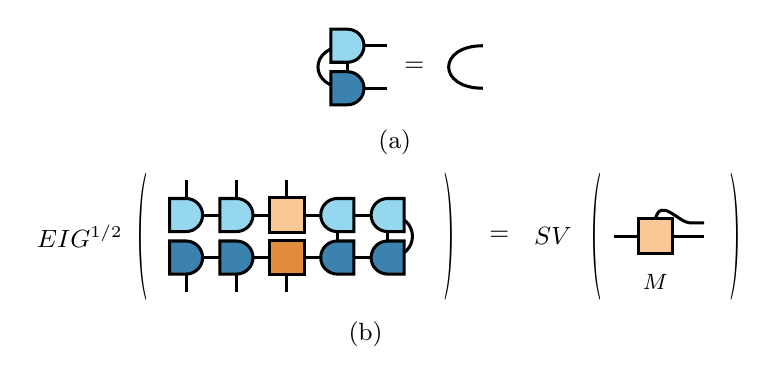
\begin{tikzpicture}[
    bond/.style={draw=black, line width=1.1pt},
    Sq/.style={rectangle, draw=black, line width=1.1pt, minimum size=4.4mm, inner sep=0pt},
    tag/.style={font=\small},
    idx/.style={font=\footnotesize},
  ]

  %% ================= (a) the canonical condition, centred =================
  \begin{scope}[xshift=2.05cm, yshift=2.15cm]
    \draw[bond] (0,\DY) .. controls (-0.50,\DY) and (-0.50,-\DY) .. (0,-\DY);
    \draw[bond] (0,\DY) -- (0,-\DY);
    \draw[bond] (0,\DY) -- (0.50,\DY);
    \draw[bond] (0,-\DY) -- (0.50,-\DY);
    \dR{0}{\DY}{ketc}
    \dR{0}{-\DY}{brac}
    \node[tag] at (0.85,0) {$=$};
    \draw[bond] (1.72,\DY) .. controls (1.14,\DY) and (1.14,-\DY) .. (1.72,-\DY);
    \node[tag] at (0.6,-0.95) {(a)};
  \end{scope}

  %% ================= (b) the RDM spectrum is local =================
  \node[tag] at (-1.35,0) {$EIG^{1/2}$};
  \node at (-0.55,0) {\bigpar{(}};

  % the reduced density matrix at a cut: left block open, right block traced
  \foreach \r/\s/\f/\g in {1/\DY/ketc/ctrk, -1/-\DY/brac/ctrb} {
    \draw[bond] (0,\s) -- ({4*\DX},\s);
  }
  \foreach \i in {0,1,2} {
    \draw[bond] (\i*\DX,\DY)  -- (\i*\DX,{\DY+\ST});
    \draw[bond] (\i*\DX,-\DY) -- (\i*\DX,{-\DY-\ST});
  }
  \foreach \i in {3,4} { \draw[bond] (\i*\DX,\DY) -- (\i*\DX,-\DY); }
  \draw[bond] ({4*\DX},\DY) .. controls ({4*\DX+0.42},\DY) and ({4*\DX+0.42},-\DY)
              .. ({4*\DX},-\DY);

  \foreach \i in {0,1} {
    \dR{\i*\DX}{\DY}{ketc}
    \dR{\i*\DX}{-\DY}{brac}
  }
  \node[Sq, fill=ctrk] at ({2*\DX},\DY)  {};
  \node[Sq, fill=ctrb] at ({2*\DX},-\DY) {};
  \foreach \i in {3,4} {
    \dL{\i*\DX}{\DY}{ketc}
    \dL{\i*\DX}{-\DY}{brac}
  }

  \node at ({4*\DX+0.78},0) {\bigpar{)}};
  \node[tag] at ({4*\DX+1.42},0) {$=$};
  \node[tag] at ({4*\DX+2.10},0) {$SV$};
  \node at ({4*\DX+2.65},0) {\bigpar{(}};

  % the orthogonality centre alone. The physical leg bends round to run parallel to the right bond:
  % the two indices are grouped, which is what turns M into a matrix for the SVD.
  \begin{scope}[xshift={(4*\DX+3.40)*1cm}]
    \draw[bond] (-0.52,0) -- (0.62,0);
    \draw[bond] (0,0.22) .. controls (0.07,0.50) and (0.30,0.17) .. (0.44,0.17) -- (0.62,0.17);
    \node[Sq, fill=ctrk] at (0,0) {};
    \node[idx, anchor=north] at (0,-0.36) {$M$};
  \end{scope}
  \node at ({4*\DX+4.42},0) {\bigpar{)}};

  \node[tag] at ({2*\DX+1.0},-1.25) {(b)};

\end{tikzpicture}
\end{document}
.
\documentclass[tikz,border=3pt]{standalone}
\usepackage{amsmath,amssymb,braket,graphicx}
\usetikzlibrary{arrows.meta,shapes.geometric}

\definecolor{ketc}{RGB}{150,215,240}
\definecolor{brac}{RGB}{60,130,175}
\definecolor{ctrk}{RGB}{250,200,150}
\definecolor{ctrb}{RGB}{225,140,60}

\newcommand{\DX}{0.64}
\newcommand{\DY}{0.27}
\newcommand{\ST}{0.44}

\newcommand{\Dhh}{0.21}   % half-height of a tensor
\newcommand{\Dbb}{0.21}   % straight body, so the D is as wide as it is tall

% D-shaped tensors centred at (#1,#2), filled #3; \dR has its flat edge left, \dL right
\newcommand{\dR}[3]{%
  \filldraw[fill=#3, draw=black, line width=1.1pt]
    ({#1-(\Dbb+\Dhh)/2},{#2-\Dhh}) -- ({#1+(\Dbb-\Dhh)/2},{#2-\Dhh})
    arc[start angle=-90, end angle=90, radius=\Dhh]
    -- ({#1-(\Dbb+\Dhh)/2},{#2+\Dhh}) -- cycle;}
\newcommand{\dL}[3]{%
  \filldraw[fill=#3, draw=black, line width=1.1pt]
    ({#1+(\Dbb+\Dhh)/2},{#2-\Dhh}) -- ({#1-(\Dbb-\Dhh)/2},{#2-\Dhh})
    arc[start angle=-90, end angle=-270, radius=\Dhh]
    -- ({#1+(\Dbb+\Dhh)/2},{#2+\Dhh}) -- cycle;}

\newcommand{\bigpar}[1]{\scalebox{1.1}[4.6]{$#1$}}

\begin{document}
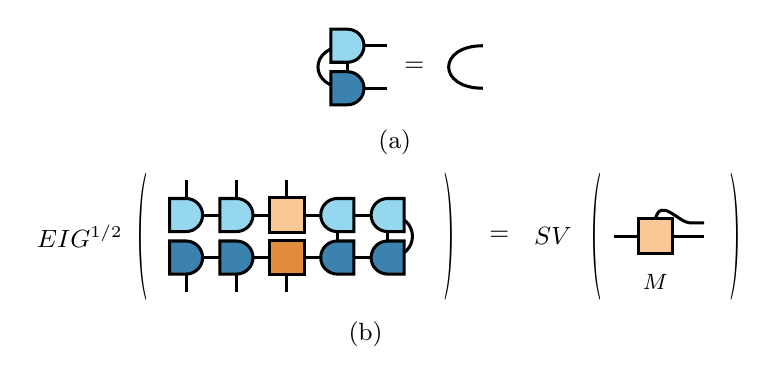
\begin{tikzpicture}[
    bond/.style={draw=black, line width=1.1pt},
    Sq/.style={rectangle, draw=black, line width=1.1pt, minimum size=4.4mm, inner sep=0pt},
    tag/.style={font=\small},
    idx/.style={font=\footnotesize},
  ]

  %% ================= (a) the canonical condition, centred =================
  \begin{scope}[xshift=2.05cm, yshift=2.15cm]
    \draw[bond] (0,\DY) .. controls (-0.50,\DY) and (-0.50,-\DY) .. (0,-\DY);
    \draw[bond] (0,\DY) -- (0,-\DY);
    \draw[bond] (0,\DY) -- (0.50,\DY);
    \draw[bond] (0,-\DY) -- (0.50,-\DY);
    \dR{0}{\DY}{ketc}
    \dR{0}{-\DY}{brac}
    \node[tag] at (0.85,0) {$=$};
    \draw[bond] (1.72,\DY) .. controls (1.14,\DY) and (1.14,-\DY) .. (1.72,-\DY);
    \node[tag] at (0.6,-0.95) {(a)};
  \end{scope}

  %% ================= (b) the RDM spectrum is local =================
  \node[tag] at (-1.35,0) {$EIG^{1/2}$};
  \node at (-0.55,0) {\bigpar{(}};

  % the reduced density matrix at a cut: left block open, right block traced
  \foreach \r/\s/\f/\g in {1/\DY/ketc/ctrk, -1/-\DY/brac/ctrb} {
    \draw[bond] (0,\s) -- ({4*\DX},\s);
  }
  \foreach \i in {0,1,2} {
    \draw[bond] (\i*\DX,\DY)  -- (\i*\DX,{\DY+\ST});
    \draw[bond] (\i*\DX,-\DY) -- (\i*\DX,{-\DY-\ST});
  }
  \foreach \i in {3,4} { \draw[bond] (\i*\DX,\DY) -- (\i*\DX,-\DY); }
  \draw[bond] ({4*\DX},\DY) .. controls ({4*\DX+0.42},\DY) and ({4*\DX+0.42},-\DY)
              .. ({4*\DX},-\DY);

  \foreach \i in {0,1} {
    \dR{\i*\DX}{\DY}{ketc}
    \dR{\i*\DX}{-\DY}{brac}
  }
  \node[Sq, fill=ctrk] at ({2*\DX},\DY)  {};
  \node[Sq, fill=ctrb] at ({2*\DX},-\DY) {};
  \foreach \i in {3,4} {
    \dL{\i*\DX}{\DY}{ketc}
    \dL{\i*\DX}{-\DY}{brac}
  }

  \node at ({4*\DX+0.78},0) {\bigpar{)}};
  \node[tag] at ({4*\DX+1.42},0) {$=$};
  \node[tag] at ({4*\DX+2.10},0) {$SV$};
  \node at ({4*\DX+2.65},0) {\bigpar{(}};

  % the orthogonality centre alone. The physical leg bends round to run parallel to the right bond:
  % the two indices are grouped, which is what turns M into a matrix for the SVD.
  \begin{scope}[xshift={(4*\DX+3.40)*1cm}]
    \draw[bond] (-0.52,0) -- (0.62,0);
    \draw[bond] (0,0.22) .. controls (0.07,0.50) and (0.30,0.17) .. (0.44,0.17) -- (0.62,0.17);
    \node[Sq, fill=ctrk] at (0,0) {};
    \node[idx, anchor=north] at (0,-0.36) {$M$};
  \end{scope}
  \node at ({4*\DX+4.42},0) {\bigpar{)}};

  \node[tag] at ({2*\DX+1.0},-1.25) {(b)};

\end{tikzpicture}
\end{document}
